\documentclass[DIV=13,fontsize=11pt]{scrartcl}
\usepackage[T1]{fontenc}
\usepackage{lmodern}
\usepackage[ngerman]{babel}
\usepackage[utf8]{inputenc}
\usepackage{csquotes}
\usepackage[hidelinks]{hyperref}
\usepackage{amsmath}
\usepackage{amssymb} 
\usepackage{listings}
\usepackage{float}
\usepackage{graphics,graphicx}
\usepackage[left=2cm, right=2cm, top=2cm, bottom=2cm, bindingoffset=1cm, includeheadfoot]{geometry}
\usepackage[onehalfspacing]{setspace}
\usepackage[backend=biber,style=numeric,maxcitenames=1,sorting=none]{biblatex}\addbibresource{bib.bib}

% aendert u.a. bei zitierungen zu et al.
\DefineBibliographyStrings{ngerman}{ 
   andothers = {et\addabbrvspace al\adddot},
   andmore   = {et\addabbrvspace al\adddot},
}

\setlength{\parindent}{0pt}

\begin{document}
% ----------------------------------------------------------------------------
\subject{Projektbericht zum Modul Data Mining Wintersemester 20221/2022}
\title{Reproduktion des Papers \\ \textit{Context-Sensitive Visualization of Deep Learning Natural Language Processing Models}\cite{dunn2021context}}
\author{Max Henze}% obligatorisch
\maketitle% verwendet die zuvor gemachte Angaben zur Gestaltung eines Titels
% ----------------------------------------------------------------------------

\section{Einleitung}

%Beschreiben sie mit ein paar Sätzen den Kontext der replizierten/reproduzierten Arbeit. 
%Es werden höchstens drei bis vier Paragraphen erwartet. Sie sollen hinreichend erklären, was das das Problem ist, das der Artikel bearbeitet, 
%warum es ein wichtiges Problem ist und das die Beiträge des replizierten/reproduzierten Artikel ist. Zitieren sie in diesem Abschnitt 
%relevante wissenschaftliche Arbeiten.
% Was ist der Beitrag des replizierten Artikels?
% Welche Teile der Arbeit wurden für die Replikation ausgewählt? Begründen Sie die Auswahl. Warum wurden andere Teile der Arbeit nicht repliziert?
% Welche neuen Erkenntnisse erwarten Sie durch die geplante Reproduktion? Was steht davon nicht in dem replizierten Artikel?
% Was ist der Beitrag bzw. sind die Beiträge Ihres Artikels über die Reproduktion der ausgewählten Arbeit?

Neuronale Netzwerke mit Transformern sind ein beliebtes Hilfsmittel in NLP und
Modelle wie BERT~\cite{devlin2018bert} oder GPT~2~\cite{radford2019language} gehören schon lange zum state-of-the-art, was durch ihre sehr guten
Ergebnisse~\cite{minaee2021deep,liu2019text,sun2019utilizing} in diversen Bereichen untermahlt wird.
Doch die Tatsache, dass Einblicke in diese sehr komplexen Modelle und ein somit besseres Verständnis für von ihnen getroffene Entscheidungen
nicht sehr einfach ist, war Anlass für \citeauthor{dunn2021context} um sich in ihrer Arbeit~\cite{dunn2021context} näher damit
zu beschäftigen. Konkret: \citeauthor{dunn2021context} entwickelten in ihrem Paper einen Ansatz zur abstufenden Visualisierung der Wichtigkeit
von Wörtern, wie sie von einem Neuronalen Netz bei der Klassifikation bewertet werden.

Ziel dieser Arbeit ist es das ganze Paper von \citeauthor{dunn2021context} zu replizieren. Es existiert kein Code und keine sonstigen Beigaben
zum Paper, sodass jegliche Replikationen aus den Wortlauten und Beschreibungen der Autoren erzeugt werden müssen.
%TODO vllt. noch neues Experiment hinzufügen ? 

Durch diese Arbeit sollen die Experimente von \citeauthor{dunn2021context} erneut verifiziert werden. Der erzeugte Code soll anderen Lesern
als Hilfestellung beim Verständnis des Papers dienen und somit eine einfache Möglichkeit bei der Erstellung weiterer Experimente geben.

\section{Umfang der Replikation/Reproduktion}
% Erklären sie die Behauptungen/Hypothesen/Experimente des Artikels, die sie für ihre Replikation/Reproduktion ausgewählt haben.
% Motivieren und begründen sie ihre Auswahl.
% Es ist sinnvoll, wenn sie sich auf die Behauptung konzentrieren, die der Hauptbeitrag des Artikels ist.
% Um den Hauptbeitrag herauszufinden, versuchen sie den Artikel in ein bis zwei Sätzen zusammenzufassen, z.B.
% \begin{quote}
%     ``This paper introduces a new activation function X that outperforms a similar activation function Y on tasks Z,V,W.''  oder

%     ``Dieser Artikel führt eine neuartige Aktivierungsfunktion X ein, welche die ähnliche Aktivierungsfunktionen Y für die Aufgaben Z,W,V deutlich verbessert.''
% \end{quote}
% Stecken sie den Umfang ihrer Replikation/Reproduktion so klar wie möglich ab.
% Die Behauptungen ihres Berichts sollten durch die Ergebnisse ihrer Experimente unterstützt oder widerlegt werden.
% Schauen sie sich zum Beispiel diese Beschreibung an:
% \begin{quote}
%     ``Contextual embedding models have shown strong performance on a number of tasks across NLP. We will run experiments evaluating two types of contextual embedding models on datasets X, Y, and Z.'' oder

%     ``Für Contextual-Embedding-Modelle wurde nachgewiesen, dass die bei einer Vielzahl von Aufgaben aus einem breiten Spektrum natürlichen Sprachverarbeitung (NLP) eine hervorragende Leistung erbringen. Wir evaluieren experimentell zwei verschiedene Arten von Contextual-Embedding-Modellen auf den Datensätzen X, Y, Z.''
% \end{quote}
% Der Umfang ist zu breit angelegt und es fehlt die Erwartung für ein klares Ergebnis.
% Schauen sie sich die nächste Beschreibung an:
% \begin{quote}
%     ``Finetuning pretrained BERT on SST-2 will have higher accuracy than an LSTM trained with GloVe embeddings.'' oder

%     ``Das Anpassen eines vortrainierten BERT-Modells für die SST-2-Aufgabe führt zu einer höheren Klassifikationsrate als ein LSTM-Modell, das für GloVe-Einbettungen trainiert wurde''
% \end{quote}
% Hier ist klarer was bei der Reproduktion/Replikation herauskommen kann. Diese Aussage könnte durch ihre Ergebnisse tatsächlich bestätigt oder widerlegt werden.

% Führen sie eindeutig die Behauptungen auf, die sie in ihrer Arbeit untersuchen.
% \begin{itemize}
%     \item Behauptung 1
%     \item Behauptung 2
%     \item Behauptung 3
% \end{itemize}

Der Umfang dieser Replikation umfasst die gesamte Arbeit von \citeauthor{dunn2021context}. Diese lässt sich zu der Aussage zusammenfassen,
dass bei der Klassifikation von Dokumenten bestimmte Wörter einen größeren Einfluss haben als andere. Dies geht mit unserer
Intuition einher, da zum Beispiel \textit{und} weniger aussagt als \textit{bombastisch} und somit letzteres den Text in einen
vermutlich eher positiven Kontext rückt.
Nun gibt es Techniken wie leave-one-out, welche über alle Token in einem Dokument durch iterieren,
das gerade betrachtete Token entfernen und dann den Text neu klassifizieren. Die Wahrscheinlichkeit, der Neuklassifikation
kann also mit der Wahrscheinlichkeit des Originaltextes verglichen werden wodurch eine gewisse
Wichtigkeit des Wortes innerhalb der Klassifikation deutlich wird. Basierend auf diesen Techniken propagieren \citeauthor{dunn2021context} nun
folgende Behauptung:

\begin{itemize}
    \item \glqq Unser Ansatz schaut auf die Kombination von Wörtern und Sätzen um deren Einfluss auf die Ausgabe des Modells zu erkennen, was zu einer Visualisierung führt, welche kontextsensitiver zum Originaltext ist.\grqq \cite{dunn2021context}
\end{itemize}

\section{Methoden}

\subsection{Modellbeschreibung}
%Beischreiben sie die Modelle, die im Originalartikel genutzt werden, einschließlich der Architektur, der Zielfunktion und der Parameter.
Bei dem in der Arbeit von \citeauthor{dunn2021context} benutztem Modell handelt es sich um ein BERT-base Modell ohne genauere Angaben.
%TODO ausfüllen 


\subsection{Datenbeschreibung}
Der im Originalartikel und dieser Replikation verwendete Datensatz ist das large Movie
Review Dataset~\cite{maas-EtAl:2011:ACL-HLT2011} der Universität Stanford.
Dieser umfasst 50.000 Dokumente mit einer Teilung in 25.000 Trainingsdokumente und 25.000 Testdokumente und kann unter
\url{https://ai.stanford.edu/~amaas/data/sentiment/} heruntergeladen werden. Dies wird im Jupyter Notebook automatisch gemacht, falls
der Datensatz noch nicht vorhanden ist.
Der Datensatz hat eine vorgegebene Ordnerstruktur, so befinden sich die Trainingsdokumente und Testdokumente in eigenen Ordnern,
wobei positive und negative Dokumente nochmals in eigene Ordner unterteilt sind. Eine Datei ist in der Struktur \texttt{x\_y.txt}
angegeben wobei x die Dokumentenid und y die Sternewertung von 0 bis 10 ist.
Die Dokumente unterscheiden sich stark in der Länge, so gibt es Dokumente mit knapp über 50 Zeichen aber auch solche mit über 13.000 Zeichen.
Die Dokumente an sich sind nicht aufbereitet, enthalten englische Altagssprache und Sonverzeichen.

\begin{figure}[H]
    \centering
    \begin{lstlisting}
        Fair drama/love story movie that focuses on the lives of 
        blue collar people finding new life thru new love.The acting 
        here is good but the film fails in cinematography,screenplay,
        directing and editing.The story/script is only average at best.
        This film will be enjoyed by Fonda and De Niro fans and by 
        people who love middle age love stories where in the coartship 
        is on a more wiser and cautious level.
        It would also be interesting for people who are 
        interested on the subject matter regarding illiteracy.......
    \end{lstlisting}
    \caption{Beispieltext eines positiven Trainingsdokuments}
\end{figure}

Zusätzlich zu der Unterteilung in Trainings- und Testdaten, wurden die Trainingsdaten wie im Originalartikel angegeben
noch in 20 Prozent Validierungsdaten geteilt.

\subsection{Hyperparameter}
%Beschreiben sie, wie sie Hyperparameter gesetzt haben. Welche Quellen haben sie für die konkreten Werte genutzt (z.B. den Forschungsartikel, Code oder sie hatten eine wohlbegründete Vermutung, educated guess).
Die im Modell einstellbaren Hyperparameter sind: Chargengröße (batch size), Lernrate, Epochenanzahl und Verlustrate des Dropout Layers.
Auch hier waren keine Angaben seitens des Originalartikels vorhanden. Daher orientierte sich die Festlegung dieser Parameter an
externen Berichten. Nur die Chargengröße orientierte sich nicht an diesen. Um ein Training auf einer Grafikkarte zu ermöglichen
musste diese verringert werden.
\textit{Tensorflow}\footnote{\url{https://www.tensorflow.org/}}, das zur Implementierung des Modells verwendete Python Package,
schlägt Werte für eine Textklassifikation mit BERT vor. Diese Vorschläge orientieren sich am selben Datensatz wie er hier Anwendung findet,
sodass diese Werte im Projekt übernommen wurden und für eine sehr gute Performance des Models sorgen. Mehr dazu im nächsten Kapitel.

Über das \textit{officials.nlp} Package wurde der AdamW~\cite{DBLP:journals/corr/abs-1711-05101} Optimierer implementiert,
welcher beim Training die Hyperparameter des Modells anpasst.

\subsection{Implementierung}
% Beschreiben sie, ob sie vorhandenen Code oder eigenen Code genutzt haben.
% Stellen sie Links zum Code bereit und beschreiben sie welche Programmiersprachen und Pakete genutzt wurden.
% Ihr Github oder Gitlab-Reposititory sollte öffentlich sein.
% Das Reposititory sollte klar dokumentiert werden.

Die Implementierung erfolgte über Python\footnote{\url{https://www.python.org/}} mit
Hilfe eines Jupyter Notebooks\footnote{\url{https://jupyter.org/}}.

Sie gliederte sich in drei große Abschnitte: Modellerzeugung, Ergebnisverarbeitung, Visualisierung.

\subsubsection{Modellerzeugung}

Die Modellerzeugung wurde mit Hilfe des \textit{tensorflow} und des \textit{official.nlp} Package bearbeitet.

Zuerst wurden die Daten in die drei Datensätze: Test, Training und Validierung unterteilt. Dies wurde mit Hilfe der
\texttt{text\_datase\_from\_directory} Funktion aus \textit{tensorflow} erzeugt. Die Ordnerstruktur der Daten ist standartisiert
und somit im richtigen Format um von der Funktion verarbeitet zu werden.

Der Encoder, also das eigentliche BERT Modell und der Preprocesser können über eine
zentrale Anlaufstelle\footnote{\url{https://tfhub.dev}} heruntergeladen werden.

\begin{figure}[H]
    \centering
    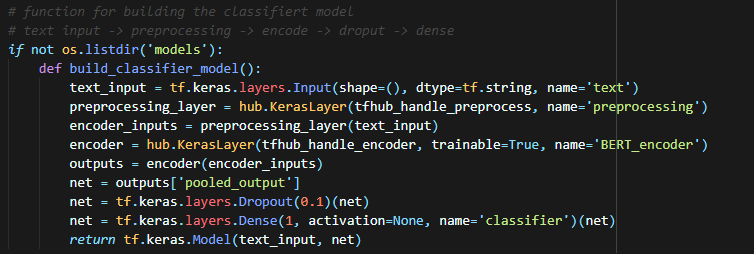
\includegraphics[width=\linewidth]{img/model_code.png}
    \caption{Funktion um das Klassifikationsmodell zu erzeugen. Es besteht aus einem Input-, Preprocessing-, Encode-, Dropout-
        und Denselayer.}
    \label{fig:model}
\end{figure}

Wie in Abbildung \ref{fig:model} zu sehen ist, wurden die einzelnen Layer mit Hilfe von \texttt{hub.KerasLayer}
(\textit{tensorflow} Package) hintereinander geschalten.

Als Lossfunktion wurde Binary Crossentropy und als Metrik die Binary Accuracy verwendet. Beide können ebenfalls über
\textit{tensorflow} geladen und verwendet werden.

Nun kann das Modell kompiliert, trainiert und dann getestet werden. Dabei ergeben sich folgende Ergebnisse:



\subsection{Aufbau der Experimente}
Erklären sie, wie sie ihre Experimente durchgeführt haben. Was für Ressourcen haben sie verwendet, z.B. GPU/CPU-Ressourcen.
Verlinken sie ihren Code und Notebooks.
%Explain how you ran your experiments, e.g. the CPU/GPU resources and provide the link to your code and notebooks. 

\subsection{Ressourcen für Berechnungen}
Beschreiben sie die Anforderungen für die Berechnungen für jedes ihrer Experimente, z.B. die Anzahl der CPU/GPU-Stunden oder die Voraussetzungen für den Hauptspeicher und GPU-Speicher.
Geben sie für Zeit und Speicher eigene Abschätzungen an, bevor die Experimente gelaufen sind und vergleichen sie dies mit den tatsächlich verbrauchten Ressourcen.
Sie müssen vor den Experimenten einplanen, dass diese Informationen auch durch ihren Code gemessen und gespeichert werden.

% Provide information on computational requirements for each of your experiments. For example, the number of CPU/GPU hours and memory requirements.
% Mention both your estimation made before running the experiments (i.e. in the proposal) and the actual resources you used to reproducing the experiments. 
% \textbf{\textit{You'll need to think about this ahead of time, and write your code in a way that captures this information so you can later add it to this section.} }


\section{Ergebnisse}
Starten sie mit einem Überblick über die Ergebnisse.
Bestätigen ihre Ergebnisse die aufgeführten Behauptungen?
Dieser Abschnitt sollte hauptsächlich Fakten nennen und so präzise wie möglich geschrieben werden.
Die Bewertung und Diskussion kann im späteren Kapitel ``Diskussion'' folgen.

% Start with a high-level overview of your results. Does your work support the claims you listed in section 2.1? Keep this section as factual and precise as possible, reserve your judgement and discussion points for the next ``Discussion'' section. 

Beschreiben sie dann detailliert jedes einzelne Ergebnis, das sie haben.
Zeigen sie wie es mit einer oder mehreren Behauptungen in Beziehung steht.
Erklären sie konkret was der Kern ihres Ergebnis ist.
Gruppieren sie die Ergebnisse in logische Abschnitte.
Beschreiben sie klar, wo sie über den Originalartikel hinausgegangen sind, wo sie zusätzliche Experimente durchgeführt haben und wie diese mit den ursprünglichen Behauptungen in Beziehung stehen.

% Go into each individual result you have, say how it relates to one of the claims, and explain what your result is. Logically group related results into sections. Clearly state if you have gone beyond the original paper to run additional experiments and how they relate to the original claims. 

Tipp 1: Drücken sie sich genau aus und verwenden sie eine klare und einfache Sprache, z.B.
\begin{quote}
    ``we reproduced the accuracy to within 1\% of reported value, that upholds the paper's conclusion that it performs much better than baselines.'' oder

    ``We konnten die Klassifikationsrate bis auf 1\% des angegebenen Werts reproduzieren. Dies unterstützt die Schlussfolgerung der Artikels, dass der Ansatz leistungsfähiger als die Baselines ist.''
\end{quote}
Oft kann man nicht die exakt gleiche numerische Zahl als Ergebnis bekommen. Deshalb müssen sie das Ergebnis bewerten, um zu entscheiden, ob ihr Ergebnis die Behauptung der Originalartikels unterstützt.
% Getting exactly the same number is in most cases infeasible, so you'll need to use your judgement call to decide if your results support the original claim of the paper. 

Tipp 2: Nutzen sie Tabellen und Abbildungen, um ihre Ergebnisse darzustellen.
% You may want to use tables and figures to demonstrate your results.

% The number of subsections for results should be the same as the number of hypotheses you are trying to verify.

\subsection{Ergebnis 1}

\subsection{Ergebnis 2}

\subsection{Zusätzliche Ergebnisse, die nicht im Originalartikel enthalten waren}
Beschreiben sie alle zusätzlichen Experimente, die über den Originalartikel hinausgehen.
Dies können Experimente zu weiteren Datenmengen sein oder sie probieren andere Methoden bzw. weitere Vereinfachungen des Modells aus oder passen die Hyperparameter an.
Beschreiben sie für jedes zusätzliche Experiment, was sie genau durchgeführt haben, was die Ergebnisse sind und diskutieren sie was diese Ergebnisse zeigen.

% Describe any additional experiments beyond the original paper. This could include experimenting with additional datasets, exploring different methods, running more ablations, or tuning the hyperparameters. For each additional experiment, clearly describe which experiment you conducted, its result, and discussions (e.g. what is the indication of the result).

\section{Diskussion}
Beschreiben sie die weiterführenden Implikationen der experimentellen Ergebnisse.
War der Originalartikel replizierbar bzw. reproduzierbar.
Falls nicht, welche Faktoren haben dazu geführt, dass die Experimente nicht reproduziert werden konnten.

% Describe larger implications of the experimental results, whether the original paper was reproducible, and if it wasn’t, what factors made it irreproducible. 

Bewerten sie, ob sie die Evidenz, die sie durch das Durchführen der Experimente erhalten haben, auch überzeugt, dass die Behauptungen des Originalartikels dadurch gestützt werden.
Diskutieren sie die Stärken und Schwächen ihres Ansatzes, vielleicht haben sie aus Zeitgründen nicht alle Experimente durchführen können, oder vielleicht haben zusätzliche Experimente durchgeführt, die den Originalartikel weiter stärken.

% Give your judgement on if you feel the evidence you got from running the code supports the claims of the paper. Discuss the strengths and weaknesses of your approach -- perhaps you didn't have time to run all the experiments, or perhaps you did additional experiments that further strengthened the claims in the paper.


\subsection{Was war einfach?}
Beschreiben sie welche Teile der Replikation/Reproduktion sich leicht umsetzen ließen.
Lief der Code der Autoren problemlos? War es aufgrund der Beschreibung im Originalartikel nicht aufwändig die Methoden zu reimplementieren?
Dieser Abschnitt soll den Lesenden zeigen, welche Teile des Originalartikels sich leicht für eigene Ansätze verwenden lässt.

% Describe which parts of your reproduction study were easy. E.g. was it easy to run the author's code, or easy to re-implement their method based on the description in the paper. The goal of this section is to summarize to the reader which parts of the original paper they could easily apply to their problem. 

Tipp: Machen sie keine pauschalen Verallgemeinerungen. Was für sie leicht ist, muss für andere nicht leicht sein. Geben sie genügend Kontext und erklären sie warum manche Sachen leicht waren, z.B. der Code hatte eine umfangreiche Dokumentation der Schnittstellen und viele Beispiele aus der Dokumentation passten zu den Experimenten im Artikel.

% Be careful not to give sweeping generalizations. Something that is easy for you might be difficult to others. Put what was easy in context and explain why it was easy (e.g. code had extensive API documentation and a lot of examples that matched experiments in papers). 

\subsection{Was war schwer?}
Beschreiben sie welche Teile ihrer Replikation/Reproduktion aufwändig oder schwierig waren oder viel mehr Zeit in Anspruch genommen haben, als sie erwarteten.
Vielleicht waren Daten nicht verfügbar, so dass sie einige Experimente nicht verifizieren konnten, oder der Code der Autoren funktionierte nicht und musste erst debugged werden.
Vielleicht dauerten auch einige Experimente zu lange und sie konnten sie deshalb nicht verifizieren.
Dieser Abschnitt soll den Lesenden zeigen, welche Teile des Originalartikels schwer wiederverwendbar sind, bzw. signifikante Zusatzarbeiten und Ressourcen erfordern.

% Describe which parts of your reproduction study were difficult or took much more time than you expected. Perhaps the data was not available and you couldn't verify some experiments, or the author's code was broken and had to be debugged first. Or, perhaps some experiments just take too much time/resources to run and you couldn't verify them. The purpose of this section is to indicate to the reader which parts of the original paper are either difficult to re-use, or require a significant amount of work and resources to verify. 

Tipp: Setzen sie sorgfältig ihre Diskussion in den richtigen Kontext, z.B. sagen sie nicht `` die Mathematik war schwer verständlich'' sondern sagen sie `` die Mathematik erfordert fortgeschrittene Kenntnisse in Analysis für das Verständnis''.

% Be careful to put your discussion in context. For example, don't say ``the math was difficult to follow,'' say ``the math requires advanced knowledge of calculus to follow.'' 

\subsection{Empfehlungen für die Replizierbarkeit / Reproduzierbarkeit}
Geben sie Empfehlungen, wie die Autoren des Originalartikels oder andere Forschende in diesem Feld die Replizierbarkeit / Reproduzierbarkeit verbessern können.

% Describe a set of recommendations to the original authors or others who work in this area for improving reproducibility.

\section{Kommunikation mit den Autoren}
Dokumentieren sie das Ausmaß (oder das Fehlen) der Kommunikation mit Autoren.
Stellen sie sicher, dass der Bericht eine faire Beurteilung der Forschungsarbeiten ist. Versuchen sie deshalb mit den Autoren Kontakt aufzunehmen.
Sie können ihnen konkrete Fragen stellen oder falls sie keine Fragen haben, den Bericht zusenden und um Feedback bitten.

% Document the extent of (or lack of) communication with the original authors. To make sure the reproducibility report is a fair assessment of the original research we recommend getting in touch with the original authors. You can ask authors specific questions, or if you don't have any questions you can send them the full report to get their feedback.



% \section{Lösungsansätze für das Problem}
% Kurze Zusammenfassung verwandter/konkurrierender Arbeiten, die das Problem auf ähnliche Weise lösen (zwei Artikel oder mehr)
% Erste Gruppe von Artikeln 
% Zweite Gruppe von Artikeln
% Kurze Zusammenfassung von Arbeiten, Methoden oder Techniken auf denen der replizierte Artikel aufbaut (zwei Artikel oder mehr)
% Erste Gruppe von Artikeln 
% Zweite Gruppe von Artikeln 
% Kurze Beschreibung des/der Ansatzes/Ansätze, die für die Replikation ausgewählt wurden.
% Offene Details, die im replizierten Artikel nicht oder unvollständig beschrieben wurden und die nicht zitierten Artikeln geklärt werden.
% Welche Details können durch die Reproduktion geklärt und ergänzt werden? Erklären Sie diese Details.
% Welche Prinzipien, Ideen, Grundlagen oder Annahmen stehen hinter dem replizierten Ansatz?



% \section{Empirische Evaluation und Replikation}
% Beschreibung der Implementierung 
% Beschreibung von einfachen Tests, die die Korrektheit der Implementierung belegen
% Beschreibung des Speicherverbrauchs und der Laufzeit-Performance der Implementierung
% Beschreibung der Ausgangsdaten
% Beschreibung der Vorverarbeitung der Daten
% Beschreibung der Replikation des/der Experiment/e
% Beschreibung von Schwierigkeiten und Problemen



% \section{Zusammenfassung}
% Ist der Ansatz gut genug, um das Problem als gelöst zu betrachten?
% Welche Schwierigkeiten des Ansatzes deckte die Replikation auf?
% Welche Forschungenrichtungen halten Sie für künftige Untersuchen für potentiell wichtig?

% \section{Entwicklung und Julia-Code}
% Implementierung Datenvorverarbeitung 
% Implementierung Modell
% Implementierung von Tests, Ausgaben, Grafiken, die Arbeitsweise und Korrektheit belegen
% Implementierung zur Auswertung offener Details im replizierten Artikel
% Implementierung des replizierten Experiments, Evaluation
% Implementierung Evaluationsauswertung



\end{document}
